\section{Announcements}
\begin{itemize}
    \item Pset \#9 is due Wednesday, November 4, at 11:59 PM (Pacific time).
    \item Pset \#10 will be released Wednesday, November 4, and is due Wednesday,
    November 11, at 11:59 PM 
\end{itemize}
\section{Goals}

By the end of this lecture, you will be able to compute the output of an LTI system to any input signal...in frequency domain.

This goal has two parts: you already know how to achieve the first part --- the convolution integral gives you the output of an LTI system to any input signal if you know the impulse response of the system. The second part is what we will focus on in this lecture: how to compute the output of an LTI system in frequency domain, and how that might be useful in engineering.

\section{Review: Output of LTI systems using convolution}
Consider a system $H$ shown in the block diagram below:
\begin{center}
\begin{tikzpicture}[scale=1, every node/.style={transform shape}]
    \node[gain] (H) {$H$};
    \node[left of=H, node distance=3cm] (x) {$x(t)$};
    \node[right of=H, node distance=3cm] (y) {$y(t)$};
    \draw[conn] (x) -- (H);
    \draw[conn] (H) -- (y);
\end{tikzpicture}
\end{center}
Note that $H$ is a notation we are using for the system. It is not a function, or a signal. It is the abstract representation of the system itself. We usually model the system using its impulse response $h(t)$. That is, the response (output) of the system when the input is $\delta(t)$ is $h(t)$. For the input $x(t)$, what is the output $y(t)$ of the system? The answer is given by the convolution integral:
\[
y(t) = x(t) * h(t) = \int_{-\infty}^{\infty} x(\tau) h(t - \tau) d\tau.
\]
This is the time-domain representation of the output of an LTI system. 
\section{Review: Breaking down signals}
We have seen many ways of breaking down signals into simpler components in this class: breaking down a signal into shifted and scaled impulses using the sifting property of the delta function, breaking down a signal into step functions, breaking down a signal into complex exponentials using Fourier series and Fourier transforms, etc. We review the last two methods below.
\subsection{Periodic signals can be broken down using Fourier series}
For a periodic signal $x(t)$ with period $T$, we can write:
\begin{equation}
    \label{eq:w10l1-fs-synthesis}
x(t) = \sum_{k=-\infty}^{\infty} a_k e^{j k \omega_0 t}, \end{equation}
where $\omega_0 = \frac{2\pi}{T}$ and 
\begin{equation}
    \label{eq:w10l1-fs-analysis}
    a_k = \frac{1}{T} \int_{T} x(t) e^{-j k \omega_0 t} dt.
\end{equation}

\subsection{Aperiodic signals can be broken down using Fourier transforms}
If a signal $x(t)$ is aperiodic, we can break it down into complex exponentials using the Fourier transform. The Fourier transform is also a representation of the signal $x(t)$ in the frequency domain (with frequency variable $\omega$ as the X-axis). We have
\begin{equation}
    \label{eq:w10l1-ft-analysis}
X(\omega) = \int_{-\infty}^{\infty} x(t) e^{-j \omega t} dt,
\end{equation}
and the inverse Fourier transform (Fourier synthesis) is given by
\begin{equation}
    \label{eq:w10l1-ft-synthesis}
x(t) = \frac{1}{2\pi} \int_{-\infty}^{\infty} X(\omega) e^{j \omega t} d\omega.
\end{equation}

\section{Computing the output of LTI systems}
We start this section with a pop-quiz where you will be asked to apply your knowledge of LTI systems (superposition) and Fourier series to compute the output of an LTI system to a periodic input signal.
\begin{popquiz}
For an LTI system, we know that the output of the system to an input $e^{j \omega t}$ is given by $H(j \omega) e^{j \omega t}$, where $H(j \omega)$ is the frequency response of the system (observe the eigenfunction property as the input appears again in the output). Using the Fourier series representation of a periodic signal, compute the output of an LTI system to a periodic input signal $x(t)$ with period $T$.
\popqsplit 
Using the Fourier series representation of $x(t)$ from \eqref{eq:w10l1-fs-synthesis}, we have
\[
x(t) = \sum_{k=-\infty}^{\infty} a_k e^{j k \omega_0 t},
\]
where $\omega_0 = \frac{2\pi}{T}$. Using the superposition property of LTI systems, the output of the system to the input $x(t)$ is given by
\[
y(t) = \sum_{k=-\infty}^{\infty} a_k H(j k \omega_0) e^{j k \omega_0 t}.
\]
The Fourier series coefficients of the output signal $y(t)$ are given by $b_k = a_k H(j k \omega_0)$.
\end{popquiz}
For a periodic signal $x(t)$ with period $T$, the output of an LTI system to the input $x(t)$ is given by
\[
y(t) = \sum_{k=-\infty}^{\infty} a_k H(j k \omega_0) e^{j k \omega_0 t},
\]
where $a_k$ are the Fourier series coefficients of $x(t)$ and $\omega_0 = \frac{2\pi}{T}$.
The Fourier series coefficients of the output signal $y(t)$ are given by
\[
b_k = a_k H(j k \omega_0).
\]
Observe how the Fourier Series coefficients of the output signal (this is the frequency domain representation of the periodic output signal) are obtained by multiplying the Fourier series coefficients of the input signal with the frequency response of the system evaluated at discrete frequencies $k \omega_0$.
\subsection{Output of LTI systems to aperiodic signals in the frequency domain}
Now, we move on to finding the output of an LTI system to aperiodic input signals. But before we jump into it, it is important to remind ourselves of the time-shifting property of the Fourier transform.
\begin{popquiz}
If the Fourier transform of a signal $x(t)$ is $X(\omega)$, prove that the Fourier transform of the time-shifted signal $x(t - t_0)$ is given by $X(\omega) e^{-j \omega t_0}$.
\popqsplit
Using the definition of the Fourier transform, we have
\[
\begin{aligned}
\mathcal{F}\{x(t - t_0)\} &= \int_{-\infty}^{\infty} x(t - t_0) e^{-j \omega t} dt.
\end{aligned}
\]
Apply the most common integration solving trick: change of variables (colloquially known as $u$-sub). Let $u = t - t_0$. Then, $du = dt$, and $t = u + t_0$. Substituting these in the integral, we get
\[
\begin{aligned}
\mathcal{F}\{x(t - t_0)\} &= \int_{-\infty}^{\infty} x(u) e^{-j \omega (u + t_0)} du \\
&= e^{-j \omega t_0} \int_{-\infty}^{\infty} x(u) e^{-j \omega u} du \\
&= e^{-j \omega t_0} X(\omega).
\end{aligned}
\]
\end{popquiz}
To write the output of an LTI system to an aperiodic input signal, we start with the convolution equation
\[
y(t) = x(t) * h(t) = \int_{-\infty}^{\infty} x(\tau) h(t - \tau) d\tau.
\]
The Fourier transform of the output signal $y(t)$ is given by using the Fourier transform equation~\eqref{eq:w10l1-ft-analysis}:
\[
\begin{aligned}
Y(\omega) &= \int_{-\infty}^{\infty} y(t) e^{-j \omega t} dt \\
&= \int_{-\infty}^{\infty} \left( \int_{-\infty}^{\infty} x(\tau) h(t - \tau) d\tau \right) e^{-j \omega t} dt \\
&= \int_{-\infty}^{\infty} x(\tau) \left( \int_{-\infty}^{\infty} h(t - \tau) e^{-j \omega t} dt \right) d\tau
\end{aligned}
\]
where we wrote the last step by interchanging the order of integration: we brought the $d\tau$ integral outside and kept all the terms involving $\tau$ inside. We kept the $t$ terms where they were and we will now integrate over $t$ first. From the previous pop-quiz, we know that
\[
\int_{-\infty}^{\infty} h(t - \tau) e^{-j \omega t} dt = H(\omega) e^{-j \omega \tau}.
\]
Substituting this in the previous equation, we get
\[
\begin{aligned}
Y(\omega) &= \int_{-\infty}^{\infty} x(\tau) H(\omega) e^{-j \omega \tau} d\tau \\
&= H(\omega) \int_{-\infty}^{\infty} x(\tau) e^{-j \omega \tau} d\tau \\
&= H(\omega) X(\omega).
\end{aligned}
\]
Thus, we have shown that the output signal (in frequency domain) is given by
\[
Y(\omega) = H(\omega) X(\omega)
\]
the product of the frequency response of the system and the Fourier transform of the input signal. Just the multiplication! No integration!

This is a VERY IMPORTANT result. For starters, it lets us compute the output of an LTI system to any input signal using simple multiplication in frequency domain. Second, it gives us insights into how different frequency components of the input signal are affected by the system. For example, if $H(\omega)$ is small for large values of $\omega$, then we know that high-frequency components of the input signal will be attenuated in the output signal. It allows us to \emph{design} systems with a desired $H(\omega)$. For example, if there are two (or however many) frequencies that I absolutely dislike (my ears hurt when I hear the screeching sound of a chalk on a blackboard of frequency $\omega_1$!). Then, I can design a system such that the frequency response $H(\omega)$ has very small values at $\omega_1$: $H(\omega_1) \approx 0$. This system will attenuate the frequency component $\omega_1$ in the output signal. Such systems are called notch filters. 

The fundamental concept we have derived above is called the Convolution Theorem (or the convolution property of Fourier transforms).

\section{Example: First-order decay systems}
A lot of things in real-life respond with a first-order decay to an impulse input. That is, if you suddenly push someone (an impulse input), they might be affected at $t=0$ but then they will slowly come to rest (decay) over time. Mathematically, the impulse response of such a system is given by
\[
h(t) = e^{-a t} u(t),
\]
where $a > 0$ is a constant that determines how fast the system decays. The unit step function $u(t)$ ensures that the impulse response is causal (the output cannot start before the input is applied at $t=0$). 

Now, what if there is a new input from a particularly annoying classmate who pushes you for a while but slowly decays their push. The input signal can be modeled as
\[
x(t) = e^{-b t} u(t),
\]
where $b > 0$ is another constant. What is the output of the system to this input signal?

To compute the output of the system to this input signal, we first compute the Fourier transforms of the input signal and the impulse response.
\[
\begin{aligned}
X(\omega) &= \int_{0}^{\infty} e^{-b t} e^{-j \omega t} dt \\
&= \int_{0}^{\infty} e^{-(b + j \omega) t} dt \\
&= \left[ \frac{e^{-(b + j \omega) t}}{-(b + j \omega)} \right]_{0}^{\infty} \\
&= \frac{1}{b + j \omega},
\end{aligned}
\]
and
\[
\begin{aligned}
H(\omega) &= \int_{0}^{\infty} e^{-a t} e^{-j \omega t} dt \\
&= \int_{0}^{\infty} e^{-(a + j \omega) t} dt \\
&= \left[ \frac{e^{-(a + j \omega) t}}{-(a + j \omega)} \right]_{0}^{\infty} \\
&= \frac{1}{a + j \omega}.
\end{aligned}
\]
Using the convolution theorem, the output of the system in frequency domain is given by
\[
Y(\omega) = H(\omega) X(\omega) = \frac{1}{(a + j \omega)(b + j \omega)}.
\]
It's that easy! Now, we can already analyze the frequency properties of the output without bothering to apply the convolution integral or the inverse Fourier transform. For example, we can see that as $\omega \to \infty$, $Y(\omega) \to 0$. Thus, high-frequency components of the input signal are attenuated in the output signal.

With the convolution theorem at hand, we can now study many many kinds of engineering systems because this is what enables many areas of electrical engineering: frequency modulation, amplitude modulation, communication systems, control systems, signal processing, image filtering, audio processing, and more! Soon\dots
\section{Examples: Filtering}
Let's start with a simple example. Consider the design of an audio processing system. So, our goal is to design $h(t)$ in time-domain (or if it is easier, we might design $H(j\omega)$ in frequency-domain) to achieve the desired output characteristics. Let's say that there is an audio input signal $x(t)$ and we only want to keep the three most dominant frequency components of the signal and remove all other frequency components in the output. If the three most dominant frequency components are at frequencies $\omega_1$, $\omega_2$, and $\omega_3$, then we can design the frequency response of the system as follows:
\[
H(j\omega) = \begin{cases}
    1, & \text{if } |\omega| \in (\omega_1 - \Delta \omega, \omega_1 + \Delta \omega) \\
    1, & \text{if } |\omega| \in (\omega_2 - \Delta \omega, \omega_2 + \Delta \omega) \\
    1, & \text{if } |\omega| \in (\omega_3 - \Delta \omega, \omega_3 + \Delta \omega) \\
    0, & \text{otherwise}
\end{cases}
\]
where \( \Delta \omega \) is a small frequency range around each dominant frequency component. This design allows only the desired frequency components to pass through while attenuating all other frequencies (because of the convolution property). 
\subsection{Filtering an audio mix}
Consider an audio signal where you have three frequency tones mixed together:
\[
x(t) = \cos(t) + \cos(5t) + \cos(100t)
\]
The three frequency components are at \( \omega_1 = 1 \) rad/s, \( \omega_2 = 5 \) rad/s, and \( \omega_3 = 100 \) rad/s. Our goal is to design a filter that only allows the frequency component at \( \omega_2 = 5 \) rad/s to pass through while attenuating the other two frequency components. We can achieve this by designing the frequency response of the audio processing system. Then, by using the convolution property, the output Fourier Transform will be the product of the input Fourier Transform and the designed frequency response. Finally, we can use the Inverse Fourier Transform to recover the time-domain output signal.

The first step is to compute the Fourier Transform of the input signal \( x(t) \). 
\begin{popquiz}
    What is the Fourier Transform of \( x(t) = \cos(\omega_0 t) \)? Start by predicting what you expect the $\cos(t)$ signal to look like in the frequency domain? Hint: It's just one frequency component. 
    % draw a cos(t) on left in time-domain and draw a delta at omega=1 and omega=-1 on right in frequency-domain with $\omega$ as x-axis on the right.
    \begin{tikzpicture}
  %----- time-domain axis -----
  \begin{axis}[
    axis lines=middle,
    xlabel={$t$},
    ylabel={$x(t)$},
    xtick={-6.2832,-3.1416,0,3.1416,6.2832},
    xticklabels={$-2\pi$,$-\pi$,$0$,$\pi$,$2\pi$},
    ytick={-1,0,1},
    ymin=-1.5, ymax=1.5,
    width=6cm,
    height=4cm,
    domain=-6.2832:6.2832,
    samples=200
  ]
    \addplot[blue, thick] {cos(deg(x))};
  \end{axis}

  %----- frequency-domain axis (impulses) -----
  \begin{axis}[
    axis lines=middle,
    xlabel={$\omega$},
    ylabel={$X(j\omega)$},
    xtick={-1,0,1},
    xticklabels={$-1$,$0$,$1$},
    ytick=\empty,
    ymin=0, ymax=1.4,
    width=6cm,
    height=4cm,
    xshift=8cm,
    clip=false
  ]
    % vertical impulse "stems" with arrowheads
    \addplot+[
      ycomb,
      blue,
      thick,
      mark=triangle*,
      mark options={scale=1.2},
    ] coordinates {(-1,1) (1,1)};
    % optional labels for amplitudes (e.g., \pi)
    %\node[above, blue] at (axis cs:-1,1) {$\pi$};
    %\node[above, blue] at (axis cs:1,1) {$\pi$};
  \end{axis}
\end{tikzpicture}

    \popqsplit 
    Intuitively, we expect the Fourier Transform of \( \cos(\omega_0 t) \) to consist of impulse at the frequency components \( \omega = \omega_0 \). However, because we work with complex exponentials, we actually have two impulses: one at \( \omega = \omega_0 \) and another at \( \omega = -\omega_0 \). The negative frequency arises due to the Euler's formula representation of cosine (which converts the complex to the real):
    \[
    \cos(\omega_0 t) = \frac{1}{2} \left( e^{j \omega_0 t} + e^{-j \omega_0 t} \right)
    \]
    So, it's clear that there is a frequency at $\omega_0$ and another frequency at $-\omega_0$.
\end{popquiz}
To see the Fourier transform of a cosine signal formally, compute the inverse Fourier Transform of the following signal:
\[ 
X(\omega) = 2 \pi \delta(\omega - \omega_0)
\]

The inverse Fourier Transform is given by:
\[
x(t) = \frac{1}{2\pi} \int_{-\infty}^{\infty} X(\omega) e^{j \omega t} d\omega
\]
(you can see the reason why we have $2\pi$ in front of the delta function --- so it cancels out with the $\frac{1}{2\pi}$ term in front of the integral in the inverse Fourier Transform equation).

Substituting \( X(\omega) = 2 \pi \delta(\omega - \omega_0) \) into the inverse Fourier Transform equation, we have:
\[
x(t) = \frac{1}{2\pi} \int_{-\infty}^{\infty} 2 \pi \delta(\omega - \omega_0) e^{j \omega t} d\omega
\]
now, using the sifting property of the delta function, we can evaluate the integral:
\[
x(t) = e^{j \omega_0 t}
\]
since the area under curve of the impulse is $1$, we get $e^{j \omega_0 t}$.

So, we have the Fourier Transform pair:
\[
X(\omega) = 2 \pi \delta(\omega - \omega_0) \quad \leftrightarrow \quad x(t) = e^{j \omega_0 t}
\]
Now, using Euler's formula, we can express the cosine function in terms of complex exponentials:
\[
\cos(\omega_0 t) = \frac{1}{2} \left( e^{j \omega_0 t} + e^{-j \omega_0 t} \right)
\]
So, the Fourier Transform of \( \cos(\omega_0 t) \) can be derived by taking the Fourier Transform of each exponential term separately and adding them together by using the linearity property of the Fourier Transform.

\[
\mathcal{F}\{ \cos(\omega_0 t) \} = \frac{1}{2} \left( \mathcal{F}\{ e^{j \omega_0 t} \} + \mathcal{F}\{ e^{-j \omega_0 t} \} \right)
\]

We get, 
\[
\mathcal{F}\{ \cos(\omega_0 t) \} = \frac{1}{2} \left( 2 \pi \delta(\omega - \omega_0) + 2 \pi \delta(\omega + \omega_0) \right) 
= \pi \left( \delta(\omega - \omega_0) + \delta(\omega + \omega_0) \right)
\]

So, now we can write $X(\omega)$ for our input signal \( x(t) = \cos(t) + \cos(5t) + \cos(100t) \):
\[
X(\omega) = \pi \left( \delta(\omega - 1) + \delta(\omega + 1) \right) + \pi \left( \delta(\omega - 5) + \delta(\omega + 5) \right) + \pi \left( \delta(\omega - 100) + \delta(\omega + 100) \right)
\]
Our goal is to design a filter that only allows the frequency component at \( \omega = 5 \) rad/s to pass through while attenuating the other two frequency components. Therefore, we can design the frequency response of the audio processing system as follows:
\[
H(j\omega) = \begin{cases}
    1, & \text{if } |\omega| \in (5 - \Delta \omega, 5 + \Delta \omega) \\
    0, & \text{otherwise}
\end{cases}
\]
where \( \Delta \omega \) is a small frequency range around \( 5 \) rad/s. Visually, this frequency response is shown in Figure~\ref{fig:frequency_response_example}.
\begin{figure}[h]
    \centering
    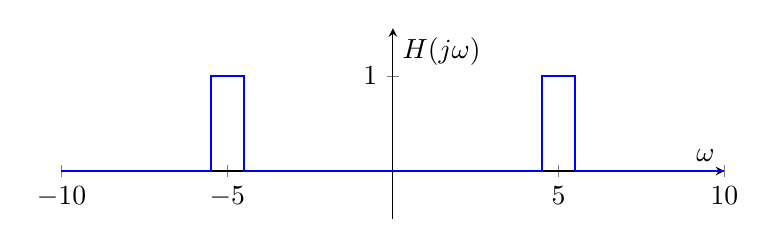
\begin{tikzpicture}
  \begin{axis}[
    axis lines=middle,
    xlabel={$\omega$},
    ylabel={$H(j\omega)$},
    xmin=-10, xmax=10,
    ymin=-0.5, ymax=1.5,
    xtick={-10,-5,0,5,10},
    xticklabels={$-10$,$-5$,$0$,$5$,$10$},
    ytick={0,1},
    width=10cm,
    height=4cm
  ]
    % Ideal two-line passband around ±5 (here width = 1: [4.5,5.5] and [-5.5,-4.5])
    \addplot[blue, thick] coordinates {
      (-10,0) (-5.5,0) (-5.5,1) (-4.5,1) (-4.5,0)
      ( 4.5,0) ( 4.5,1) ( 5.5,1) ( 5.5,0) (10,0)
    };
  \end{axis}
\end{tikzpicture}

    \caption{Frequency response of the designed filter.}
    \label{fig:frequency_response_example}
\end{figure}
The output Fourier Transform \( Y(\omega) \) is given by the product of the input Fourier Transform \( X(\omega) \) and the designed frequency response \( H(j\omega) \):
\[
Y(\omega) = X(\omega) H(j\omega)
= \pi \left( \delta(\omega - 5) + \delta(\omega + 5) \right)
\]
because all other impulses are multiplied by zero.

Finally, we can use the Inverse Fourier Transform to recover the time-domain output signal \( y(t) \):
\[
y(t) = \frac{1}{2\pi} \int_{-\infty}^{\infty} Y(\omega) e^{j \omega t} d\omega
= \frac{1}{2\pi} \int_{-\infty}^{\infty} \pi \left( \delta(\omega - 5) + \delta(\omega + 5) \right) e^{j \omega t} d\omega
\]
\[
= \frac{1}{2} \left( e^{j 5 t} + e^{-j 5 t} \right) = \cos(5t)
\]
Thus, the output signal \( y(t) \) contains only the frequency component at \( \omega = 5 \) rad/s, as desired.

\section{Recommended reading and practice problems}
Section 4.5.1 in Oppenheim and Willsky, 2nd edition is an interesting section to read to learn more about the applications of Fourier transforms in communication.
